%!TEX TS-program = xelatex
%!TEX encoding = UTF-8 Unicode

\documentclass[11pt,reqno]{amsart}
\usepackage{graphicx}

\synctex=1

% showframe, showcrop
\usepackage[driver=xetex,paperwidth=7in,paperheight=10in,text={5.5in,8.5in},left=0.65in,top=0.75in,headheight=0.25in,headsep=0.4in,footskip=0.4in]{geometry}
%\usepackage{subfigure}
\usepackage{amsmath,amssymb,amsthm}
%\usepackage[usenames,dvipsnames]{color}
%\usepackage[xetex,cmyk]{xcolor}
\usepackage[xetex]{xcolor}
\usepackage{framed}
%\usepackage{sidecap}
\usepackage{natbib}
%\usepackage{makeidx}
%\usepackage{amsmidx}
\citeindextrue
\usepackage{alltt}
\usepackage{marginnote}
%\usepackage{endnote}
%\usepackage{endnotes}
\usepackage{todonotes}
\usepackage{array}
\usepackage{booktabs}
\usepackage{setspace}
\usepackage{hyperref}

%\definecolor{shadecolor}{gray}{.90}%
\definecolor{shadecolor}{rgb}{0.95,0.95,0.99}%
%\definecolor{shadecolor}{cmyk}{0.0712,0.0344,0,0}%
\definecolor{tintedcolor}{gray}{0.80}%
\definecolor{mygray}{gray}{0.05}%
\definecolor{myblue}{rgb}{0.1,0.2,0.8}%
%\definecolor[named]{myblue}{cmyk}{0.95,0.43,0,0}%PMS 285+

%\bibpunct[, ]{(}{)}{,}{a}{}{,}

\DeclareMathOperator{\var}{var}
\DeclareMathOperator{\cov}{cov}
\DeclareMathOperator{\E}{E}
\DeclareMathOperator{\logit}{logit}

% redefine chapter heading
%\makeatletter
%\def\@makechapterhead#1{\global\topskip 7.5pc\relax \begingroup \fontsize{\@xivpt}{18}\bfseries\centering
%\ifnum\c@secnumdepth>\m@ne \leavevmode \hskip-\leftskip \rlap{\vbox to\z@{\vss
%\centerline{\normalsize\mdseries \uppercase\@xp{\chaptername}\enspace\thechapter}
%\vskip 3pc}}\hskip\leftskip\fi #1\par \endgroup
%\skip@34\p@ \advance\skip@-\normalbaselineskip \vskip\skip@ }
%\makeatother
%\makeatletter
%\def\@makechapterhead#1{\global\topskip 7.5pc\relax \begingroup \fontsize{\@xivpt}{18}\bfseries\noindent
%\ifnum\c@secnumdepth>\m@ne \leavevmode \hskip-\leftskip \rlap{\vbox to\z@{\vss
%\vskip 3pc}}\hskip\leftskip\fi {\fontsize{48pt}{50pt}\selectfont \color{myblue} \thechapter \hspace{12pt}}\begin{minipage}[b]{4.5in}\fontsize{17pt}{19pt}\selectfont \color{myblue} #1\end{minipage}\par \endgroup
%\skip@34\p@ \advance\skip@-\normalbaselineskip \vskip\skip@ \noindent\rule{\linewidth}{0.5mm}\vskip\skip@}
%\makeatother
%
%% redefine chapter* (without number)
%\makeatletter
%\def\@makeschapterhead#1{\global\topskip 7.5pc\relax \begingroup \fontsize{\@xivpt}{18}\bfseries\noindent
%\ifnum\c@secnumdepth>\m@ne \leavevmode \hskip-\leftskip \rlap{\vbox to\z@{\vss
%\vskip 3pc}}\hskip\leftskip\fi \begin{minipage}[b]{4.5in}\fontsize{17pt}{19pt}\selectfont \color{myblue} #1\end{minipage}\par \endgroup
%\skip@34\p@ \advance\skip@-\normalbaselineskip \vskip\skip@ \noindent\rule{\linewidth}{0.5mm}}
%\makeatother

% redefine section to be larger
%\makeatletter 
%\renewcommand\section{\@startsection{section}{1}
%\z@{.7\linespacing\@plus\linespacing}{.5\linespacing}
%{\large\bfseries\centering}}
%\makeatother

\makeatletter 
\renewcommand\section{\@startsection{section}{1}
\z@{.7\linespacing\@plus\linespacing}{.5\linespacing}
{\large\bfseries\centering\color{myblue}}}
\makeatother

% redefine subsection to remove indent
%\makeatletter 
%\renewcommand\subsection{\@startsection{subsection}{2}
%\normalparindent{.5\linespacing\@plus.7\linespacing}{-.5em}%
%{\normalfont\normalsize\bfseries}}
%\makeatother

\makeatletter 
\renewcommand\subsection{\@startsection{subsection}{2}
\z@{.5\linespacing\@plus.7\linespacing}{-.5em}%
{\normalfont\normalsize\bfseries}}
\makeatother

% redefine subsubsection to have some space above it, like subsection:
\makeatletter 
\renewcommand\subsubsection{\@startsection{subsubsection}{3}
\normalparindent{.5\linespacing\@plus.7\linespacing}{-.5em}%
{\normalfont\normalsize\itshape}}
\makeatother

% redefine numbering to include section
%\renewcommand{\thefigure}{\thesection.\arabic{figure}}
%\renewcommand{\theequation}{\thesection.\arabic{equation}}
%\renewcommand{\thesection}{\thesection.\arabic{section}}

%\numberwithin{equation}{chapter}
\newcounter{codesnip}[section]
%\newcommand{\codenum}{\addtocounter{codesnip}{1}\marginnote{\textsf{\tiny R code\\\vspace{-3pt}\small\thechapter.\arabic{codesnip}}}[20pt]}
\newcommand{\codenum}{\addtocounter{codesnip}{1}\immediate\write\tempfile{## R code \thesection.\arabic{codesnip}}\marginnote{{\footnotesize R code\\\vspace{-3pt}\small\thesection.\arabic{codesnip}}}[-6pt]}

\newcommand{\codeboxb}{\vspace{-4pt}\begin{shaded}\codenum\vspace{-2pt}\small}
\newcommand{\codeboxe}{\end{shaded}}
\newcommand{\outputboxb}{\small}
\newcommand{\outputboxe}{\normalsize}

\newcommand{\codeboxbT}{\vspace{-4pt}\begin{shaded}\codenum\vspace{-2pt}\footnotesize}
\newcommand{\outputboxbT}{\footnotesize}

\newcommand{\figscale}{0.75} % scale of default R graphics

% "rethinking" sections
\newenvironment{rethinking}[1]
{\begin{shaded}\small\noindent\textbf{Rethinking: {#1}}}
{\end{shaded}}

% "overthinking" sections
\newenvironment{overthinking}[1]
{\vspace{6pt}\begin{spacing}{0.95}\noindent\textcolor{myblue}{\rule{5.5in}{0.5pt}}\\\small\noindent\textbf{Overthinking: {#1}}}
{~\newline\textcolor{myblue}{\rule{5.5in}{0.5pt}}\end{spacing}\vspace{6pt}}

%%%%%%%%%%%%%%%%%%
% new verbatim environment 'VerbSaver' that writes code to file
\newwrite\tempfile

\usepackage{verbatim}
\makeatletter
\newwrite\Code@out % temp file for writing out and reading back in for display

\newcommand\VerbSaver{\obeylines\expandafter\VerbSaverArg\noexpand}

\newcommand\VerbSaverArg[1][code.txt]{%
    \gdef\FName{xcodetempx.txt}%
    \begingroup
        \@bsphack%
        \immediate\openout\Code@out\FName%
        \let\do\@makeother\dospecials%
        \catcode`\^^M\active%
        \def\verbatim@processline{%
            \immediate\write\tempfile{\the\verbatim@line}
            \immediate\write\Code@out{\the\verbatim@line}}%
        \verbatim@start}

\def\endVerbSaver{%
    \immediate\write\tempfile{}
    \immediate\closeout\Code@out\@esphack
    \endgroup
    \verbatiminput{\FName}}

\makeatother
% end of VerbSaver stuff
%%%%%%%%%%%%%%%%%%%%%%%%%%%

%%%%%%%%%%%%%%%%
% various convenience commands follow

% ref shortcuts
\newcommand{\figref}[1]{{\textsc{\color{myblue}Figure~\ref{#1}}}}
\newcommand{\figrefpp}[1]{{\textsc{Figure~\ref{#1}} (page~\pageref{#1})}}

% new end notes that contain hyperlinks back to source page
%\newcommand{\noteend}[2]{\endnote{#2 [\pageref{#1}]}\label{#1}}
%\newcommand{\noteend}[2]{\endnote{~\hypertarget{#1 anchor}~#2 [\pageref{#1}]}\hyperlink{#1 anchor}{$^\star$}\label{#1}}
\newcommand{\noteend}[2]{\hendnote{~\hypertarget{#1 anchor}~#2 [\pageref{#1}]}{#1 anchor}\label{#1}}

% glossary term formatting
\newcommand{\gterm}[1]{{\textsc{\textbf{\textcolor{myblue}{#1}}}}\index{#1}}
\newcommand{\gtermalt}[2]{{\textsc{\textbf{\textcolor{myblue}{#1}}}}\index{#2}}

% some maths shortcuts
\newcommand{\mr}{\mathrm}
%\newcommand{\flab}[1]{\text{\textsf{\textsc{\small{\textcolor{mygray}{#1}}}}}}
\newcommand{\flab}[1]{\tag*{\textsf{\textsc{\small{\textcolor{mygray}{[#1]}}}}}}
\newcommand{\clab}[1]{\tag*{{\texttt{\small{\textcolor{mygray}{#1}}}}}}
\newcommand{\pmat}[1]{\begin{pmatrix} #1 \end{pmatrix}}
\newcommand{\bmat}[1]{\begin{bmatrix} #1 \end{bmatrix}}
\newcommand{\ttilde}{\textasciitilde}
\newcommand{\ttx}[1]{\texttt{#1}}

%\usepackage{hyperendnotes}

% typefaces

\usepackage{mathspec,xltxtra,xunicode}
\defaultfontfeatures{Mapping=tex-text}
\setsansfont[Scale=MatchLowercase,Mapping=tex-text]{Helvetica}
%\setmonofont[Scale=0.88]{Andale Mono}
\setmonofont[Scale=0.85,Mapping=tex-text-sq]{Source Code Pro}

% Goudy typefaces
%\setromanfont[Scale=1.05,Ligatures={Common}]{Goudy Oldstyle Std}
%\setmathrm[Scale=1.05]{Goudy Oldstyle Std}
%\setmathfont(Digits,Latin)[Scale=1.05]{Goudy Oldstyle Std}

% Dante typefaces
%\setromanfont[Scale=1.05,Ligatures={Common}]{Dante MT Std}
%\setmathrm[Scale=1.05]{Dante MT Std}
%\setmathfont(Digits,Latin)[Scale=1.05]{Dante MT Std}

% Minion typefaces
\setromanfont[Scale=1.0,Ligatures={Common}]{Minion Pro}
\setmathrm[Scale=1.0]{Minion Pro}
\setmathfont(Digits,Latin)[Scale=1.0]{Minion Pro}

% Caslon typefaces
%\setromanfont[Scale=1.0,Ligatures={Common}]{Adobe Caslon Pro}
%\setmathrm[Scale=1.0]{Adobe Caslon Pro}
%\setmathfont(Digits,Latin)[Scale=1.0]{Adobe Caslon Pro}

% Jenson typefaces
%\setromanfont[Scale=1.1,Ligatures={Common}]{Adobe Jenson Pro}
%\setmathrm[Scale=1.1]{Adobe Jenson Pro}
%\setmathfont(Digits,Latin)[Scale=1.1]{Adobe Jenson Pro}

\usepackage{upquote}

\usepackage{fix-cm}

% fix quotes in verbatim text
%\makeatletter
%\let \@sverbatim \@verbatim
%\def \@verbatim {\@sverbatim \verbatimplus}
%{\catcode`'=13 \gdef \verbatimplus{\catcode`'=13 \chardef '=13 }} 
%\makeatother

%\makeindex{index-a}
\makeindex

\begin{document}

% file output for code blocks
\immediate\openout\tempfile=code.txt

% title page hacks
\cleardoublepage
\thispagestyle{empty}
%\setcounter{page}{0}

\title[rethinking version 1.57]{\texttt{\Large rethinking}\\An \textsf{\large R} package for fitting and manipulating Bayesian models\\Version 1.57}
\author{Richard McElreath}
%\address{Department of Anthropology and Center for Population Biology, UC Davis, Davis CA 95616 USA.}
%\email{mcelreath@ucdavis.edu}
%\date{\today}
\maketitle

%\begin{center}
%Depends: \texttt{rstan}, \texttt{coda}, \texttt{mvtnorm}, \texttt{MASS}, \texttt{parallel}, \texttt{methods}
%\end{center}

%\newpage

\setcounter{tocdepth}{2}
{%\small
\tableofcontents
}

\section{Overview}

The \texttt{rethinking} \textsf{R} package began as an instructional aid for a PhD course on applied Bayesian statistics. It has since grown into much more. Its motivation is to provide (1)  a very flexible modeling syntax that closely resembles typical mathematical notation and (2) access to both \emph{maximum a posteriori} (MAP) and Hamiltonian Monte Carlo (HMC, provided by \texttt{rstan}) for model fitting. As a result, \texttt{rethinking} can specify many more types of models than a package like \texttt{MCMCglmm} can, while also using much better sampling algorithms, as provided by \texttt{rstan}.

%But probably the greatest advantage of this interface over other MCMC interfaces is that it forces full model specifications, so you must know the model to fit it. While convenient, packages like \ttx{lme4} make it easy for users to never learn the assumptions behind their models. 

The package also provides tools for extracting and processing posterior samples and predictions, computing WAIC and DIC criteria for model comparison, and construction of posterior prediction model ensembles. Finally, there is a function \texttt{glimmer} that translates mixed model formulas in \texttt{lme4}'s \texttt{glmer} syntax into the model definitions needed to use \texttt{rethinking}'s HMC model fitting functions. The main purpose of \ttx{glimmer} is to help the user understand the model implied by a \ttx{lme4} formula. Specifying models directly with \ttx{rethinking} formulas is more flexible.

This manual is an introduction to the \ttx{rethinking} package, but not a guide to doing Bayesian statistical inference. If you are not yet familiar with conventions of applied Bayesian statistics, beginning with a textbook is a better idea. 

\subsection{Installation}

The \texttt{rethinking} package is not on CRAN. %This is because \texttt{rstan} is not on CRAN, and \texttt{rethinking} depends upon \texttt{rstan}. Also CRAN imposes a tremendous number of pointless requirements on package authors, many of which cater to very old hardware and system specifications, or merely the whims of the gatekeeper. It's not worth my time, to be honest.
Luckily it is still very easy to install \texttt{rethinking}. There are two steps. 

First, install \texttt{rstan}. It is available at \texttt{mc-stan.org}. Many users will have to install a C compiler, before they can successfully install \texttt{rstan}. The Stan website has platform specific instructions for acquiring and installing a C compiler. In my experience, there are two common platform-specific obstacles.
\begin{itemize}
\item Windows: After downloading the \texttt{RTools} installer wizard, run it by right-clicking on it and choosing ``Run as administrator.'' Then near the end of the install, be sure to check the box for setting the system \texttt{PATH} variable. This will allow your \textsf{R} install to see the compiler.
\item Mac OS X: After installing Xcode, be sure to run it once and agree to the license. Some users experience an error later when trying to compile \texttt{rstan} that states ``\texttt{llvm-g++-4.2: command not found}.'' If you get this message, it may indicate that \textsf{R} is looking for the wrong compiler; it should be using \texttt{clang++}, not \texttt{llvm-g++}. You can trick \textsf{R} into seeing the correct compiler by opening the Terminal and issuing these three lines of code, one after another:
\begin{verbatim}
cd /usr/bin
sudo ln -fs clang llvm-gcc-4.2
sudo ln -fs clang++ llvm-g++-4.2
\end{verbatim}
\end{itemize}
Once the compiler is installed, continue with the instructions on the \texttt{mc-stan.org} website. After \texttt{rstan} finishes compiling, it's a good idea to close \textsf{R} and restart it.

The second step is to install \texttt{rethinking} itself. You have two options. You can download it from Github or from the author's repository. To install from Github, use these commands within \textsf{R}:
\codeboxb
\begin{VerbSaver}
install.packages(c('devtools','coda','mvtnorm'))
library(devtools)
install_github("rmcelreath/rethinking")
\end{VerbSaver}
\codeboxe
\noindent Or to install from the repository:
\codeboxb
\begin{VerbSaver}
install.packages(c('coda','mvtnorm'))
options(repos=c(getOption('repos'),rethinking='http://xcelab.net/R'))
install.packages('rethinking',type='source')
\end{VerbSaver}
\codeboxe

Once both \texttt{rstan} and \texttt{rethinking} are installed, you can access the in-system help files with:
\codeboxb
\begin{VerbSaver}
library(rethinking)
help(package=rethinking)
\end{VerbSaver}
\codeboxe
\noindent Like most \textsf{R} documentation, those help pages provide technical reference but do not really stand on their own. The textbook that accompanies the \texttt{rethinking} package, \emph{Statistical Rethinking: A Bayesian Course with R Examples}, provides many examples of its use. The remainder of this manual provides additional technical documentation and concise examples of different model families that can be specified and fit.


\subsection{\texttt{map}: \emph{Maximum a posteriori} fitting}

The \texttt{map} function provides an interface for \emph{maximum a posteriori} fitting, usually abbreviated ``MAP.'' MAP fitting uses optimization to search for the minimum of the log-posterior, as defined by a model. The parameter values that minimize the log-posterior possess maximum posterior probability, so these are the MAP parameter values. \texttt{map} finds the MAP values, using \textsf{R}'s built-in \texttt{optim}, and then approximates the curvature near them using the Hessian. This effectively assumes a multivariate Gaussian posterior distribution. 

\subsubsection{Model formulas}
A statistical model is specified for \texttt{map} by using a list of formulas. For example, here is a simple linear regression:
\codeboxb
\begin{VerbSaver}
a_map_formula <- alist(
    y ~ dnorm(mu,sigma),
    mu <- a + b*x,
    a ~ dnorm(0,100),
    b ~ dnorm(0,1),
    sigma ~ dunif(0,10)
)
\end{VerbSaver}
\codeboxe
\noindent The above corresponds to this model, in standard mathematical notation:
\begin{align*}
	y_i &\sim \mr{Normal}(\mu_i,\sigma)\\
	\mu_i &= \alpha + \beta x_i\\
	\alpha &\sim \mr{Normal}(0,100)\\
	\beta &\sim \mr{Normal}(0,1)\\
	\sigma &\sim \mr{Uniform}(0,10)
\end{align*}
\texttt{map} uses the formula list to build a function that computes the log-posterior for any combination of parameter values. It then passes that function to \texttt{optim}, which searches for the MAP. 

For example:
\codeboxb
\begin{VerbSaver}
data(cars)

# define model
cars_formula <- alist(
    dist ~ dnorm(mu,sigma),
    mu <- a + b*speed,
    a ~ dnorm(0,100),
    b ~ dnorm(0,10),
    sigma ~ dunif(0,50)
)

# pass to map
cars_map <- map( cars_formula , data=cars )

# default show information
show(cars_map)
\end{VerbSaver}
\codeboxe
\outputboxb
\begin{verbatim}
Maximum a posteriori (MAP) model fit

Formula:
dist ~ dnorm(mu, sigma)
mu <- a + b * speed
a ~ dnorm(0, 100)
b ~ dnorm(0, 10)
sigma ~ dunif(0, 50)

MAP values:
         a          b      sigma 
-17.400714   3.921415  15.068462 

Log-likelihood: -206.58 
\end{verbatim}
\outputboxe

\subsubsection{Initial values}
As with many optimization algorithms, \texttt{map} needs initial values for all parameters in order to begin searching. If explicit initial values are omitted, as in the above example, then \texttt{map} will sample random initial values from the priors. Initial values can be specified with a named \texttt{start} list.

It is possible to omit priors for parameters. In that case, a flat (usually improper) prior is implied and the user must also specify a starting value for the parameter. For example:
\codeboxb
\begin{VerbSaver}
cars_formula2 <- alist(
    dist ~ dnorm(mu,sigma),
    mu <- a + b*speed
)
start_list <- list(
    a=mean(cars$dist),
    b=0,
    sigma=sd(cars$dist)
)
cars_mle <- map( cars_formula2 , data=cars , start=start_list )
summary(cars_mle)
\end{VerbSaver}
\codeboxe
\outputboxb
\begin{verbatim}
        Mean StdDev   5.5% 94.5%
a     -17.59   6.62 -28.17 -7.01
b       3.93   0.41   3.28  4.58
sigma  15.07   1.51  12.66 17.48
\end{verbatim}
\outputboxe
Since the priors are flat in the example above, these estimates correspond to a maximum likelihood solution with quadratic standard errors.

\subsubsection{Link functions}
\texttt{map} understands link functions in conventional form. For example, here is a binomial model with logit link:
\codeboxb
\begin{VerbSaver}
data(UCBadmit)
UCBadmit$male <- ifelse(UCBadmit$applicant.gender=="male",1,0)
ucb_formula <- alist(
    admit ~ dbinom(applications,p),
    logit(p) <- a + b*male,
    a ~ dnorm(0,10),
    b ~ dnorm(0,1)
)
ucb_map <- map( ucb_formula , data=UCBadmit )
\end{VerbSaver}
\codeboxe

\subsubsection{Vector parameters}

\texttt{map} can construct vectors of parameters, using index variables. For example:
\codeboxb
\begin{VerbSaver}
# convert dept factor to integer index variable
UCBadmit$dept_id <- coerce_index(UCBadmit$dept)

# formula
ucb_formula2 <- alist(
    admit ~ dbinom(applications,p),
    logit(p) <- a[dept_id] + b*male,
    a[dept_id] ~ dnorm(0,10),
    b ~ dnorm(0,1)
)

ucb_map2 <- map( ucb_formula2 , data=UCBadmit )

precis(ucb_map2,depth=2)
\end{VerbSaver}
\codeboxe
\outputboxb
\begin{verbatim}
      Mean StdDev  5.5% 94.5%
a[1]  0.68   0.10  0.52  0.84
a[2]  0.64   0.12  0.45  0.82
a[3] -0.58   0.07 -0.70 -0.46
a[4] -0.61   0.09 -0.75 -0.48
a[5] -1.06   0.10 -1.22 -0.90
a[6] -2.62   0.16 -2.88 -2.37
b    -0.10   0.08 -0.23  0.03
\end{verbatim}
\outputboxe
A unique intercept estimate is return for each unique value in \texttt{dept\_id}.

\subsubsection{Custom densities}
Since \texttt{map} constructs a function for the log-posterior directly from the formula list, any \textsf{R} density function can, in principle, be used for a likelihood or prior. This includes custom functions written by the user.

\subsection{\texttt{map2stan}: Hamiltonian Monte Carlo}

The other model fitting interface is \texttt{map2stan}, which compiles the same type of formula lists into Stan models that can be fit using Hamiltonian Monte Carlo. This allows a wide range of multilevel and mixed effects models to be fit. 

Good practice when compiling models through \texttt{map2stan} includes:
\begin{enumerate}
\item Do not use any variable names with dots ``.'' in them. Stan does not allow dots in variable or parameter names. \texttt{map2stan} will convert any dots to underscores ``\_'', but mismatches between internal names and the original data will persist and lead to potential errors down the pipeline. Better to rename all variables and parameters at the start.
\item All data must be numeric. Remove any character or factor data from the data frame, or rather pass a minimal list of data to \texttt{map2stan} that omits any character or factor data.
\end{enumerate}
For example, here is a varying intercepts binomial regression:
\codeboxb
\begin{VerbSaver}
data(UCBadmit)

# construct 'male' dummy variable
UCBadmit$male <- ifelse(UCBadmit$applicant.gender=="male",1,0)

# convert dept factor to integer index variable
UCBadmit$dept_id <- coerce_index(UCBadmit$dept)

# formula
ucb_formula3 <- alist(
    admit ~ dbinom(applications,p),
    logit(p) <- a[dept_id] + b*male,
    a[dept_id] ~ dnorm(a_bar,sigma),
    b ~ dnorm(0,1),
    a_bar ~ dnorm(0,10),
    sigma ~ dcauchy(0,2.5)
)

ucb_stan <- map2stan( ucb_formula3 , data=UCBadmit , 
    iter=2000 , warmup=1000 , chains=1 ,
    refresh=500 )
\end{VerbSaver}
\codeboxe
\outputboxb
\begin{verbatim}
TRANSLATING MODEL 'admit ~ dbinom(applications, p)' FROM Stan CODE TO C++ CODE NOW.
COMPILING THE C++ CODE FOR MODEL 'admit ~ dbinom(applications, p)' NOW.

SAMPLING FOR MODEL 'admit ~ dbinom(applications, p)' NOW (CHAIN 1).

Iteration:    1 / 2000 [  0%]  (Warmup)
Iteration:  500 / 2000 [ 25%]  (Warmup)
Iteration: 1000 / 2000 [ 50%]  (Warmup)
Iteration: 1001 / 2000 [ 50%]  (Sampling)
Iteration: 1500 / 2000 [ 75%]  (Sampling)
Iteration: 2000 / 2000 [100%]  (Sampling)
#  Elapsed Time: 0.049535 seconds (Warm-up)
#                0.043325 seconds (Sampling)
#                0.09286 seconds (Total)


#  Elapsed Time: 3e-06 seconds (Warm-up)
#                2.8e-05 seconds (Sampling)
#                3.1e-05 seconds (Total)

Computing WAIC
Constructing posterior predictions
[ 1000 / 1000 ]
Aggregated binomial counts detected. Splitting to 0/1 outcome for WAIC calculation.
Warning messages:
1: In map2stan(ucb_formula3, data = UCBadmit, iter = 2000, warmup = 1000,  :
  Renaming variable 'applicant.gender' to 'applicant_gender' internally.
You should rename the variable to remove all dots '.'
2: In FUN(c("dept", "applicant_gender", "admit", "reject", "applications",  :
  data with name dept is not numeric and not used
3: In FUN(c("dept", "applicant_gender", "admit", "reject", "applications",  :
  data with name applicant_gender is not numeric and not used
4: In FUN(c("dept", "applicant_gender", "admit", "reject", "applications",  :
  data with name dept is not numeric and not used
5: In FUN(c("dept", "applicant_gender", "admit", "reject", "applications",  :
  data with name applicant_gender is not numeric and not used
\end{verbatim}
\outputboxe
The model has sampled correctly, but the warnings at the end indicate both the renaming of internal dots to underscores and the complaints about non-numeric data.

\subsubsection{Stan distribution names}

You can use Stan's internal distribution names, rather than \textsf{R} names, when defining \ttx{map2stan} models. For example, the previous model can be defined equivalently:
\codeboxb
\begin{VerbSaver}
# formula
ucb_formula4 <- alist(
    admit ~ binomial(applications,p),
    logit(p) <- a[dept_id] + b*male,
    a[dept_id] ~ normal(a_bar,sigma),
    b ~ normal(0,1),
    a_bar ~ normal(0,10),
    sigma ~ cauchy(0,2.5)
)
\end{VerbSaver}
\codeboxe

\subsubsection{Accessing samples}
Extract the samples into a named list of parameters with:
\codeboxb
\begin{VerbSaver}
post <- extract.samples(ucb_stan)
str(post)
\end{VerbSaver}
\codeboxe
\outputboxb
\begin{verbatim}
 $ a    : num [1:1000, 1:6] 0.682 0.601 0.86 0.649 0.695 ...
 $ b    : num [1:1000(1d)] -0.1716 -0.0766 -0.1984 -0.0691 -0.1067 ...
 $ a_bar: num [1:1000(1d)] -1.282 -0.303 -0.416 -0.928 -0.568 ...
 $ sigma: num [1:1000(1d)] 1.815 2.536 1.1 0.851 1.148 ...
\end{verbatim}
\outputboxe
Note that the vector of parameters \texttt{a} is returned as a matrix, with samples in rows and parameters in columns. Matrix parameters (not shown) are similarly returned as arrays, with samples in the first dimension.

\subsubsection{Accessing the internal Stan code}
The Stan code that was compiled for sampling is available with \texttt{stancode}:
\codeboxb
\begin{VerbSaver}
stancode(ucb_stan)
\end{VerbSaver}
\codeboxe
\outputboxb
\begin{verbatim}
data{
    int<lower=1> N;
    int<lower=1> N_dept_id;
    int admit[N];
    int applications[N];
    int dept_id[N];
    real male[N];
}
parameters{
    vector[N_dept_id] a;
    real b;
    real a_bar;
    real<lower=0> sigma;
}
model{
    vector[N] p;
    sigma ~ cauchy( 0 , 2.5 );
    a_bar ~ normal( 0 , 10 );
    b ~ normal( 0 , 1 );
    a ~ normal( a_bar , sigma );
    for ( i in 1:N ) {
        p[i] <- a[dept_id[i]] + b * male[i];
    }
    admit ~ binomial_logit( applications , p );
}
generated quantities{
    vector[N] p;
    real dev;
    dev <- 0;
    for ( i in 1:N ) {
        p[i] <- a[dept_id[i]] + b * male[i];
    }
    dev <- dev + (-2)*binomial_logit_log( admit , applications , p );
}
\end{verbatim}
\outputboxe
The generated quantities block is used to automatically compute DIC for each model. WAIC is also computed, but all calculations are done outside of Stan.

\subsubsection{Diagnostics}
Summary information for a \texttt{map2stan} model fit includes the per-parameter chain diagnostics \texttt{n\_eff}, the number of effective samples, and \texttt{Rhat}, the Gelman-Rubin convergence diagnostic.
\codeboxb
\begin{VerbSaver}
precis(ucb_stan,depth=2)
\end{VerbSaver}
\codeboxe
\outputboxb
\begin{verbatim}
       Mean StdDev lower 0.89 upper 0.89 n_eff Rhat
a[1]   0.68   0.10       0.53       0.83   552    1
a[2]   0.63   0.11       0.43       0.78   481    1
a[3]  -0.58   0.07      -0.70      -0.46   848    1
a[4]  -0.62   0.09      -0.77      -0.49   633    1
a[5]  -1.06   0.10      -1.22      -0.90  1000    1
a[6]  -2.61   0.15      -2.83      -2.36   847    1
b     -0.09   0.08      -0.21       0.04   413    1
a_bar -0.58   0.63      -1.58       0.38   483    1
sigma  1.48   0.57       0.73       2.18   447    1
\end{verbatim}
\outputboxe
You can also check for divergent iterations:
\codeboxb
\begin{VerbSaver}
divergent(ucb_stan)
\end{VerbSaver}
\codeboxe
\outputboxb
\begin{verbatim}
[1] 0
\end{verbatim}
\outputboxe
There were no divergent iterations in this example, but \texttt{map2stan} automatically monitors divergent iterations and warns the user if any occur. 

In addition to \ttx{divergent}, you can use \ttx{dashboard} to get a more complete report of sampler parameters. For example:
\codeboxb
\begin{VerbSaver}
sp <- dashboard(ucb_stan)
\end{VerbSaver}
\codeboxe
\noindent This plot is shown:
\begin{center}
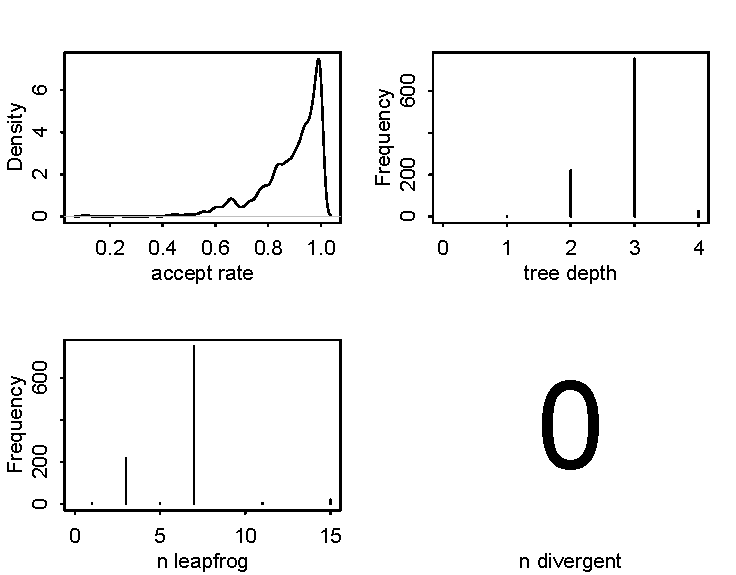
\includegraphics[width=4in]{figures/fig_dashboard.pdf}
\end{center}
And the object \ttx{sp} contains a matrix of the per-sample diagnostics.


\subsubsection{Control parameters}

Stan's control parameters can be modified by using an optional named \texttt{control} list. For example, \texttt{control=list(adapt\_delta=0.95)} sets the target acceptance rate to 95\%. See \texttt{?stan} for details.

\subsubsection{Trace plots}
To view the trace plot for all parameters:
\codeboxb
\begin{VerbSaver}
plot(ucb_stan)
\end{VerbSaver}
\codeboxe

\begin{center}
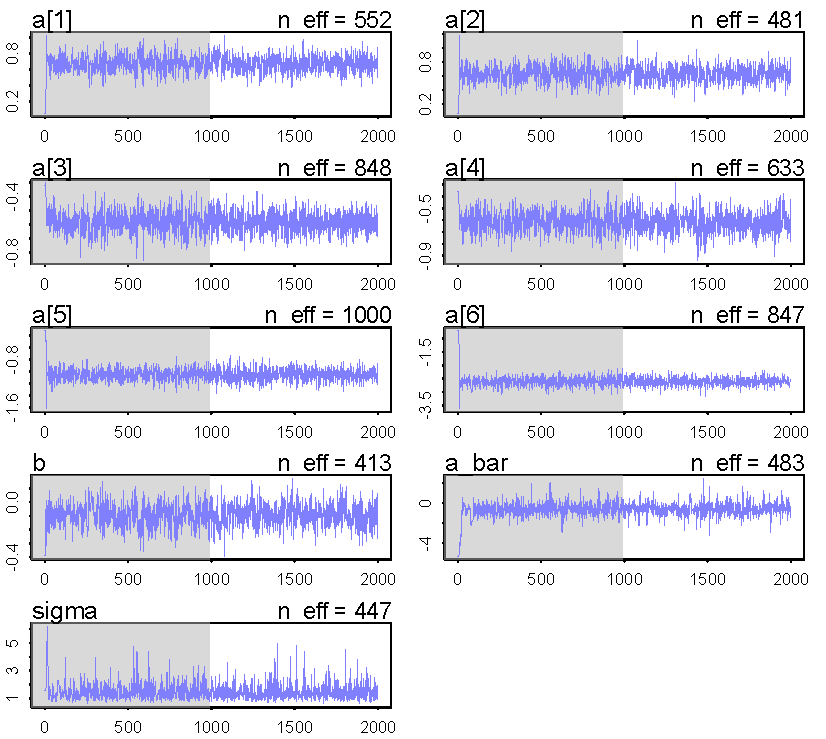
\includegraphics[width=5in]{figures/fig_traceplot.pdf}
\end{center}
Gray regions indicate warmup samples. Multiple chains are display in different colors (not shown). See \ttx{plot.map2stan} for more details and additional options. See also \ttx{pairs.map2stan} for a pairs plot method.

\subsubsection{Parameter constraints}
\texttt{map2stan} will guess some parameter constraints. For example, the standard deviation for a Gaussian likelihood or prior is automatically set to a lower bound of zero, ``\texttt{<lower=0>}'' in Stan's language. 

Additional custom parameter constraints can be specified using the \texttt{constraints} named list. For example, to redundantly specify a positive constraint on a parameter \texttt{sigma}, use \texttt{constraints=list(sigma="lower=0")}. To specify both a lower and upper bound, use \texttt{constraints=list(sigma="lower=0,upper=10")}.

As always with Stan models, it is important that the constraints on a parameter match the constraints on its prior. Otherwise, you might open a black hole or a portal to another dimension.


\subsubsection{Parameter types}
Stan is a statically typed language, and \texttt{map2stan} guesses the correct type for each parameter. If you need to manually specify a parameter type, you can use a named \texttt{types} list. For example, to define a matrix \texttt{Rho} as a correlation matrix, you could use \texttt{types=list(Rho="corr\_matrix")}.

\subsubsection{Parallel chains}
To run multiple chains in parallel on multiple cores, use the optional \texttt{cores} argument. For example:
\codeboxb
\begin{VerbSaver}
ucb_stan_4chains <- map2stan( ucb_formula3 , data=UCBadmit , 
    iter=2000 , warmup=1000 , chains=4 , cores=3 ,
    refresh=-1 )
\end{VerbSaver}
\codeboxe
\noindent The model will be pre-compiled and then the \texttt{parallel} package will be used to parallelize the chains across the number of specified cores. A single fit model object with samples from all chains will be returned. The \texttt{refresh=-1} argument above turns off the sampling progress display.

If you are experiencing crashes when parallelizing chains this way, it's probably because you are running \textsf{R} in a graphical interface, either the application from CRAN or RStudio. If you run \textsf{R} instead from the Terminal/Command Prompt, not only will those crashes stop, but it will use less memory, be more responsive, and allow you to run any number of different \textsf{R} sessions on your computer simultaneously. Graphical interfaces are so 20th century.

\subsection{Posterior predictions with \texttt{link} and \texttt{sim}}

Once you have a model fit with \texttt{map} or \ttx{map2stan}, you can process the samples directly by using \ttx{extract.samples}. For a \ttx{map} model, this draws samples from the multivariate Gaussian posterior defined by the MAP values and the variance-covariance matrix defined by the Hessian. For a \ttx{map2stan} model, this just copies the Stan samples (post-warmup) into a named list. Note that the Stan samples will be permuted, such that the chains are mixed and sequential samples are not autocorrelated. If you want the samples in the order they were drawn and split by chain (how they appear in the trace plots), see \texttt{?rstan::extract}.

There are two convenience tools, however, that make working with model predictions easier. The first is \ttx{link}, which produces posterior values of linear models. The second is \ttx{sim}, which simulates posterior predictions. This section provides an introduction to each.

\subsubsection{\ttx{link}}
This function computes the value of each linear model at each sample from the posterior. Inverse link functions are applied, so that the value of each left-hand symbol is returned. For example, in a logistic regression, the linear model will appear like this:
\outputboxb
\begin{verbatim}
logit(p) <- a + b * x
\end{verbatim}
\outputboxe
The function \texttt{link} will return the value of \ttx{p} for each sample from the posterior, not \ttx{logit(p)}. By default, the data used to fit model are used in calculation. But an optional \ttx{data} argument allows computing linear model values over any new prediction set you like.

Here's an example, using a varying intercepts logistic regression:
\codeboxb
\begin{VerbSaver}
data(chimpanzees)
d <- list( 
    pulled_left = chimpanzees$pulled_left ,
    prosoc_left = chimpanzees$prosoc_left ,
    condition = chimpanzees$condition ,
    actor = as.integer( chimpanzees$actor )
)
m <- map2stan(
    alist(
        pulled_left ~ dbinom(1,p),
        logit(p) <- a_actor[actor] + (bp + bpc*condition)*prosoc_left,
        a_actor[actor] ~ dnorm( a , sigma_actor ) ,
        a ~ dnorm(0,10),
        bp ~ dnorm(0,10),
        bpc ~ dnorm(0,10),
        sigma_actor ~ dcauchy(0,1)
    ) ,
    data=d, iter=6000 , chains=3 , cores=3 , refresh=-1 )

p <- link(m,n=2000)
str(p)
\end{VerbSaver}
\codeboxe
\outputboxb
\begin{verbatim}
 num [1:2000, 1:504] 0.199 0.373 0.265 0.28 0.382 ...
\end{verbatim}
\outputboxe
The result is a matrix, with samples on rows and observations in columns. This set of data consists of 504 observations. By using \ttx{n=2000} in the call to \ttx{link}, we ask for 2000 samples from the posterior. If you use \ttx{n=0}, you will get as many samples as Stan returned (9000 in this case).

To compute values for new data, just construct a new data frame. You need to specify values for all of the predictor variables. This includes all index variables. But outcome variables are not needed. So for example to compute posterior predictions for actor \#4 across all four treatments:
\codeboxb
\begin{VerbSaver}
new_data <- data.frame(
    actor = 4,
    prosoc_left = c(1,0,1,0),
    condition = c(1,1,0,0)
)
p <- link(m,data=new_data)
str(p)
\end{VerbSaver}
\codeboxe
\outputboxb
\begin{verbatim}
 num [1:1000, 1:4] 0.501 0.244 0.509 0.542 0.354 ...
\end{verbatim}
\outputboxe

Now what do you do with all of these linear model values? Anything you like. But the most common task is to summarize them. To compute means and 90\% highest posterior density intervals for each observation (column):
\codeboxb
\begin{VerbSaver}
p_mean <- apply(p,2,mean)
p_HPDI <- apply(p,2,HPDI,prob=0.9)
rbind(p_mean,p_HPDI)
\end{VerbSaver}
\codeboxe
\outputboxb
\begin{verbatim}
            [,1]      [,2]      [,3]      [,4]
p_mean 0.4222182 0.2680967 0.4516272 0.2680967
|0.9   0.2964644 0.1792636 0.3289030 0.1792636
0.9|   0.5415335 0.3519525 0.5679774 0.3519525
\end{verbatim}
\outputboxe

When there is more than one linear model, \ttx{link} will return a named list of matrices, one for each linear model symbol. For example, recoding the previous model so that it has two linear models:
\codeboxb
\begin{VerbSaver}
m2 <- map2stan(
    alist(
        pulled_left ~ dbinom(1,p),
        logit(p) <- a_actor[actor] + BP*prosoc_left,
        BP <- bp + bpc*condition,
        a_actor[actor] ~ dnorm( a , sigma_actor ) ,
        a ~ dnorm(0,10),
        bp ~ dnorm(0,10),
        bpc ~ dnorm(0,10),
        sigma_actor ~ dcauchy(0,1)
    ) ,
    data=d, iter=6000 , chains=3 , cores=3 , refresh=-1 )

p <- link(m2,n=2000)
str(p)
\end{VerbSaver}
\codeboxe
\outputboxb
\begin{verbatim}
List of 2
 $ p : num [1:2000, 1:504] 0.316 0.347 0.472 0.409 0.43 ...
 $ BP: num [1:2000, 1:504] 0.964 0.221 0.667 0.376 0.852 ...
\end{verbatim}
\outputboxe
The first matrix \ttx{p} is just like before, because it uses the values of the second, \ttx{BP}, in its own calculations. 

\subsubsection{\ttx{sim}}

The function \ttx{link} produces posterior distributions of linear models. To simulate observations that average over these posterior distributions, use \ttx{sim}. Here's an example, continuing with the model from the previous section.
\codeboxb
\begin{VerbSaver}
sim_pulls <- sim(m,data=new_data)
str(sim_pulls)
\end{VerbSaver}
\codeboxe
\outputboxb
\begin{verbatim}
 int [1:1000, 1:4] 0 0 1 0 0 0 0 0 0 1 ...
\end{verbatim}
\outputboxe
Rows are individual simulations and columns are observations. There are four here, because again we used the four treatments in \ttx{new\_data} from the previous section. All of these simulations produced 0 or 1, because this is a logistic regression. The average value in each column should be pretty close to corresponding value in \ttx{p\_mean} from the previous section:
\codeboxb
\begin{VerbSaver}
sim_mean <- apply(sim_pulls,2,mean)
cbind(sim_mean,p_mean)
\end{VerbSaver}
\codeboxe
\outputboxb
\begin{verbatim}
     sim_mean    p_mean
[1,]    0.441 0.4222182
[2,]    0.283 0.2680967
[3,]    0.420 0.4516272
[4,]    0.254 0.2680967
\end{verbatim}
\outputboxe

What \ttx{sim} does is identify the likelihood function in the model formula and then use the corresponding random distribution function to simulate from it. So in this case the \ttx{dbinom} likelihood is converted to \ttx{rbinom}. So if there is no random distribution function corresponding the likelihood you named in the formula definition, \ttx{sim} will not work.

\subsubsection{Posterior validation with \ttx{postcheck}}

A quick but unattractive comparison of raw data with posterior predictive distributions can be plotted with \ttx{postcheck}. This function just calls \ttx{link} and \ttx{sim} for a fit model and then plots observations on the horizontal axis and values on the vertical. It uses automatic paging, in the event there are many observations to show. The number of observations on each page is controlled by the \ttx{window} argument. See \ttx{?postcheck} for details.

Here's an example, using a varying intercepts (over-dispersed) Poisson model with log-link:
\codeboxb
\begin{VerbSaver}
data(Kline)
Kline$log_pop <- log(Kline$population)
Kline$id <- 1:10
m <- map2stan(
    alist(
        total_tools ~ dpois(lambda),
        log(lambda) <- a + a_society[id] + b*log_pop,
        a_society[id] ~ dnorm(0,sigma),
        a ~ dnorm(0,10),
        b ~ dnorm(0,1),
        sigma ~ dcauchy(0,2.5)
    ),
    data=Kline , chains=3 , core=3 , refresh=-1 )
postcheck(m)
\end{VerbSaver}
\codeboxe

\begin{center}
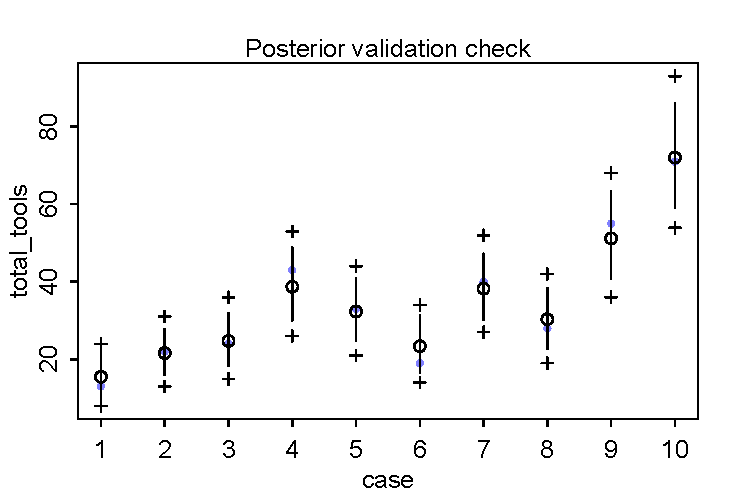
\includegraphics[scale=0.8]{figures/fig_postcheck_Kline.pdf}
\end{center}
Each case on the horizontal is a row in the data. The vertical axis is a count scale, implied by the Poisson likelihood in the model definition. Each blue point is a raw data value. Each open circle is a posterior mean prediction. The vertical line segments are 89\% posterior intervals of the mean prediction. Finally, the $+$ marks show the 89\% interval of simulated observations (from \ttx{sim} output). 

\subsubsection{Counter-factual predictions with \ttx{link} and \ttx{sim}}

It is often more useful to plot smooth counter-factual posterior predictions across a range of a predictor variable. Here's an example, using the same data as the example just above, but with a simpler model:
\codeboxb
\begin{VerbSaver}
m <- map2stan(
    alist(
        total_tools ~ dpois(lambda),
        log(lambda) <- a + b*log_pop,
        a ~ dnorm(0,10),
        b ~ dnorm(0,1)
    ),
    data=Kline , chains=1 , warmup=500 , iter=1e4 )

log_pop.seq <- seq(from=6,to=13,length.out=30)
new_data <- data.frame(log_pop=log_pop.seq)

lambda <- link(m,data=new_data,n=9000)
lambda.mean <- apply(lambda,2,mean)
lambda.HPDI <- apply(lambda,2,HPDI)
tt.sim <- sim(m,data=new_data,n=9000)
tt.HPDI <- apply(tt.sim,2,HPDI)

plot( total_tools ~ log_pop , data=Kline , pch=16 , col=rangi2 )
lines( log_pop.seq , lambda.mean )
shade( lambda.HPDI , log_pop.seq )
shade( tt.HPDI , log_pop.seq )
\end{VerbSaver}
\codeboxe
\noindent This is the result:
\begin{center}
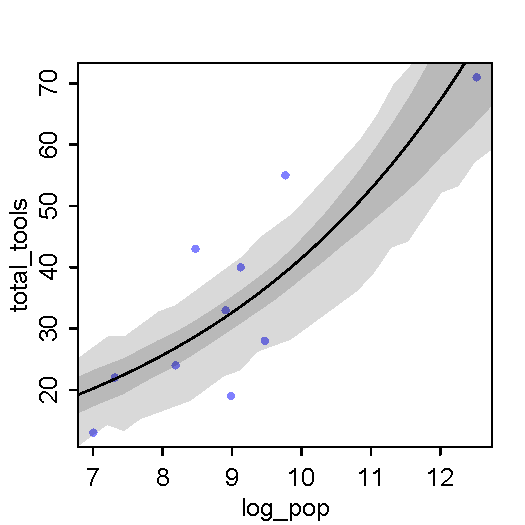
\includegraphics[scale=0.8]{figures/fig_Kline_counterfactual.pdf}
\end{center}
Note that the lighter shaded region, the simulated Poisson observation interval, is jagged. This is because it is a count outcome, so only integers are simulated. You can see this in the raw simulations:
\codeboxb
\begin{VerbSaver}
str(tt.sim)
\end{VerbSaver}
\codeboxe
\outputboxb
\begin{verbatim}
 int [1:9000, 1:30] 12 8 13 16 25 14 15 17 12 16 ...
\end{verbatim}
\outputboxe
One thing that is easy to appreciate from the counterfactual plot above is that the predictions are under-dispersed, relative to the data.

\subsection{WAIC/LOO/DIC model comparison and averaging}

The \ttx{rethinking} package provides \ttx{DIC}, \ttx{WAIC}, and \ttx{LOO} methods to compute the Deviance Information Criterion (DIC), Widely Applicable Information Criterion (WAIC), and Pareto-smoothed importance sampling Leave-One-Out cross-validation (LOO) from posterior samples for both \ttx{map} and \ttx{map2stan} model fits. The convenience functions \ttx{compare} and \ttx{ensemble} then simplify the process of comparing sets of models and constructing prediction ensembles using model weights based upon any of these criteria. Both \ttx{compare} and \ttx{ensemble} default to use WAIC. The textbook contains a lot more detail on these metrics and how the ensembles are constructed. Examples follow.

\subsubsection{\ttx{compare}}

The \ttx{compare} function accepts a series of fit \ttx{map} or \ttx{map2stan} models. It computes WAIC (or DIC) for each and then constructs a table that expedites comparison. Here's an example, constructing three models fit to the same data. These data and models are detailed in Chapter~7 of the textbook.
\codeboxb
\begin{VerbSaver}
data(rugged)
# remove cases with missing values
d <- rugged[ complete.cases(rugged$rgdppc_2000) , ]
d$log_gdp <- log(d$rgdppc_2000)
dlist <- list(
    log_gdp = d$log_gdp,
    rugged = d$rugged,
    africa = d$cont_africa
)

# intercept-only model
m1 <- map2stan(
    alist(
        log_gdp ~ dnorm(mu,sigma),
        mu <- a,
        a ~ dnorm(0,100),
        sigma ~ dcauchy(0,2.5)
    ),
    data=dlist , 
    warmup=1000 , iter=5000 , chains=2 , cores=2 , refresh=-1 )
    
# model with terrain ruggedness
m2 <- map2stan(
    alist(
        log_gdp ~ dnorm(mu,sigma),
        mu <- a + bR*rugged,
        a ~ dnorm(0,100),
        bR ~ dnorm(0,10),
        sigma ~ dcauchy(0,2.5)
    ),
    data=dlist , 
    warmup=1000 , iter=5000 , chains=2 , cores=2 , refresh=-1 )

# model with Africa indicator
m3 <- map2stan(
    alist(
        log_gdp ~ dnorm(mu,sigma),
        mu <- a + bA*africa,
        a ~ dnorm(0,100),
        bA ~ dnorm(0,10),
        sigma ~ dcauchy(0,2.5)
    ),
    data=dlist , 
    warmup=1000 , iter=5000 , chains=2 , cores=2 , refresh=-1 )

# model with both terrain ruggedness and Africa indicator
# note vector prior notation for both coefficients
m4 <- map2stan(
    alist(
        log_gdp ~ dnorm(mu,sigma),
        mu <- a + bR*rugged + bA*africa,
        a ~ dnorm(0,100),
        c(bR,bA) ~ dnorm(0,10),
        sigma ~ dcauchy(0,2.5)
    ),
    data=dlist , 
    warmup=1000 , iter=5000 , chains=2 , cores=2 , refresh=-1 )

# model with interaction of terrain ruggedness and Africa indicator
m5 <- map2stan(
    alist(
        log_gdp ~ dnorm(mu,sigma),
        mu <- a + bR*rugged + bA*africa + bRA*rugged*africa,
        a ~ dnorm(0,100),
        c(bR,bA,bRA) ~ dnorm(0,10),
        sigma ~ dcauchy(0,2.5)
    ),
    data=dlist , 
    warmup=1000 , iter=5000 , chains=2 , cores=2 , refresh=-1 )
\end{VerbSaver}
\codeboxe
\noindent You may want to verify that the chains for each model sampled correctly. Now we can invoke \ttx{compare}:
\codeboxb
\begin{VerbSaver}
compare(m1,m2,m3,m4,m5)
\end{VerbSaver}
\codeboxe
\outputboxb
\begin{verbatim}
    WAIC pWAIC dWAIC weight    SE   dSE
m5 469.6   5.3   0.0   0.88 14.89    NA
m3 474.2   2.5   4.6   0.09 14.70  7.48
m4 476.2   4.3   6.5   0.03 15.01  6.86
m1 537.1   1.4  67.5   0.00 12.88 15.48
m2 539.6   2.6  69.9   0.00 12.99 15.47
\end{verbatim}
\outputboxe
The columns are:
\begin{itemize}
\item \ttx{WAIC}: The WAIC value of each model, sorted from small (better) to large (worse)
\item \ttx{pWAIC}: The ``effective'' number of parameters for each model. This is a measure of the model's flexibility in fitting the sample.
\item \ttx{dWAIC}: Difference between each WAIC and the smallest WAIC in the set.
\item \ttx{weight}: The Akaike weight of each model in the set, conditional on the set.
\item \ttx{SE}: The estimated standard error of each WAIC.
\item \ttx{dSE}: The standard error of the different between each WAIC and the smallest WAIC in the set. Often useful to compare these values to each corresponding \ttx{dWAIC}.
\end{itemize}
The full \ttx{dSE} matrix, for a pairs of models, is available from the \ttx{dSE} slot of the invisible result that \ttx{compare} produces:
\codeboxb
\begin{VerbSaver}
compare_table <- compare(m1,m2,m3,m4,m5)
compare_table@dSE
\end{VerbSaver}
\codeboxe
\outputboxb
\begin{verbatim}
           m1         m2        m3        m4        m5
m1         NA  0.5317339 14.918201 15.154642 15.482533
m2  0.5317339         NA 14.819779 15.080354 15.473666
m3 14.9182006 14.8197790        NA  3.041996  7.483212
m4 15.1546423 15.0803543  3.041996        NA  6.855100
m5 15.4825326 15.4736656  7.483212  6.855100        NA
\end{verbatim}
\outputboxe

A crude visual representation of the information in the \ttx{compare} table is available using \ttx{plot}:
\codeboxb
\begin{VerbSaver}
plot(compare(m1,m2,m3,m4,m5))
\end{VerbSaver}
\codeboxe
\begin{center}
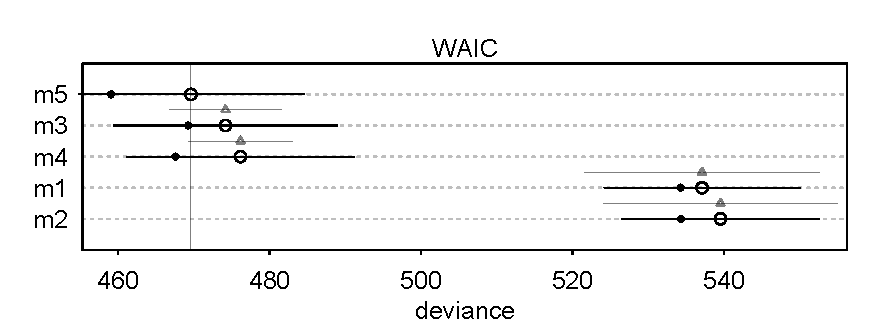
\includegraphics[scale=0.7]{figures/fig_compare.pdf}
\end{center}
The solid points are in-sample deviance values (not shown in the table, but implicitly equal to \ttx{WAIC}--2\ttx{pWAIC}). The open points are the \ttx{WAIC} values. Dark line segments on each row show plus-and-minus one standard error of WAIC. The points and gray line segments between rows show the \ttx{dWAIC} and \ttx{dSE} values.

\subsubsection{\ttx{ensemble}}

Model selection is often unwise, because of high variance in information criteria and the loss of model uncertainty. Model averaging often performs better. This means however averaging predictions, not parameter values. One way to do this is to construct a mix of posterior predictions weighted by Akaike weights. The \ttx{ensemble} function operates similarly to \ttx{link} and \ttx{sim} and automates this procedure.

Continuing with the example from just above, let's construct an ensemble of counter-factual posterior predictions. We need to visualize predictions for a nation in Africa and for a nation not in Africa. I'll show the code for one of these. Changing the value of the \ttx{africa} indicator in the data will produce the alternative plot.
\codeboxb
\begin{VerbSaver}
rugged.seq <- seq(from=0,to=7,length.out=30)
new_data <- data.frame(
    africa = 1, # imaginary nation in Africa
    rugged = rugged.seq
)

# change n argument to change number of samples used and smooth results
m1to5_ensemble <- ensemble(m1,m2,m3,m4,m5,data=new_data,n=3000)
\end{VerbSaver}
\codeboxe
\noindent The result, stored here in \ttx{m1to5\_ensemble}, contains two named matrices, \ttx{link} and \ttx{sim}, each corresponding to the model-averaged output of each simpler function. These matrices are summarized and plotted just like the simpler examples.
\codeboxb
\begin{VerbSaver}
mu.mean <- apply( m1to5_ensemble$link , 2 , mean )
mu.HPDI <- apply( m1to5_ensemble$link , 2 , HPDI )

# extract just raw data with same africa value as new_data
africa_val <- new_data$africa[1]
plot_data <- d[ d$cont_africa==africa_val , c("log_gdp","rugged") ]
plot( log_gdp ~ rugged , data=plot_data , pch=16 , col=rangi2 )
mtext( concat("africa=",africa_val) )

# overlay counter-factual predictions
lines( rugged.seq , mu.mean )
shade( mu.HPDI , rugged.seq )
\end{VerbSaver}
\codeboxe
\noindent Here are both results, for \ttx{africa=1} and \ttx{africa=0}:
\begin{center}
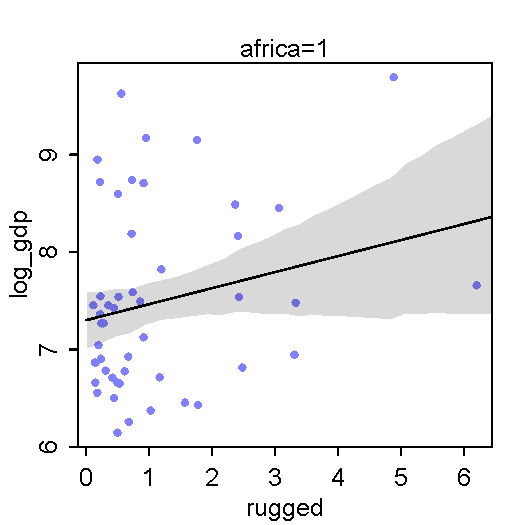
\includegraphics[scale=0.7]{figures/fig_africa1.pdf}~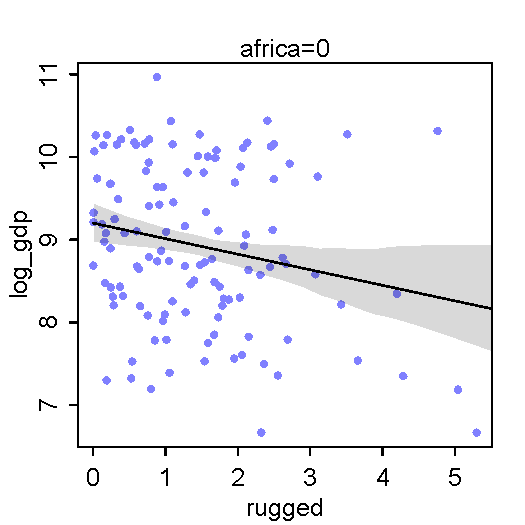
\includegraphics[scale=0.7]{figures/fig_africa0.pdf}
\end{center}
Since model \ttx{m5} has more than 75\% of the Akaike weight, it dominates predictions. But notice the asymmetric uncertainty in the slope in the righthand plot. This arise from including the lower-ranked models in the ensemble. In particular, model \ttx{m3} is second-ranked, and it ignores \ttx{rugged} completely.


\subsection{Missing data imputation with \texttt{map2stan}}

\ttx{map2stan} supports basic automated Bayesian imputation, much like BUGS and JAGS. Normally, data with missing values (\ttx{NA}) will prevent a model from running. Here's an example:
\codeboxb
\begin{VerbSaver}
data(milk)
d <- list(
    kcal = milk$kcal.per.g,
    log_mass = log(milk$mass),
    neocortex = milk$neocortex.perc/100
)
m <- map2stan(
    alist(
        kcal ~ dnorm(mu,sigma),
        mu <- a + bM*log_mass + bN*neocortex,
        a ~ dnorm(0,100),
        c(bM,bN) ~ dnorm(0,10),
        sigma ~ dcauchy(0,2.5)
    ),
    data=d , warmup=500 , iter=2500 , chains=3 , cores=3 , refresh=-1 )
\end{VerbSaver}
\codeboxe
\outputboxb
\begin{verbatim}
Error in map2stan(alist(kcal ~ dnorm(mu, sigma), mu <- a + bM * log_mass +  : 
  Variable 'neocortex' has missing values (NA) in:
a + bM * log_mass[i] + bN * neocortex
Either remove cases with NA or declare a distribution to use for imputation.
\end{verbatim}
\outputboxe
As the error message states, there are missing values in \ttx{neocortex}. We must either remove all the cases with missing values (this is what most of the automated tools in \textsf{R} do automatically and dangerously) or either provide a distribution for imputation. The second option means to state a distribution for the predictor variable \ttx{neocortex}. Like this:
\codeboxb
\begin{VerbSaver}
m2 <- map2stan(
    alist(
        kcal ~ dnorm(mu,sigma),
        mu <- a + bM*log_mass + bN*neocortex,
        neocortex ~ dnorm(mu_N,sigma_N),
        mu_N ~ dnorm(0,10),
        sigma_N ~ dcauchy(0,1),
        a ~ dnorm(0,100),
        c(bM,bN) ~ dnorm(0,10),
        sigma ~ dcauchy(0,2.5)
    ),
    data=d , warmup=500 , iter=2500 , chains=3 , cores=3 , refresh=-1 )
\end{VerbSaver}
\codeboxe
\noindent After a bunch of messages, the posterior distribution will contain one parameter for each missing value in \ttx{neocortex}:
\codeboxb
\begin{VerbSaver}
precis(m2,depth=2)
\end{VerbSaver}
\codeboxe
\outputboxb
\begin{verbatim}
                      Mean StdDev lower 0.89 upper 0.89 n_eff Rhat
neocortex_impute[1]   0.63   0.05       0.55       0.71  4864    1
neocortex_impute[2]   0.63   0.05       0.54       0.70  3855    1
neocortex_impute[3]   0.62   0.05       0.53       0.70  3391    1
neocortex_impute[4]   0.65   0.05       0.58       0.73  4291    1
neocortex_impute[5]   0.70   0.05       0.62       0.78  5253    1
neocortex_impute[6]   0.66   0.05       0.58       0.73  5285    1
neocortex_impute[7]   0.69   0.05       0.61       0.76  5339    1
neocortex_impute[8]   0.70   0.05       0.62       0.77  5533    1
neocortex_impute[9]   0.71   0.05       0.64       0.79  4730    1
neocortex_impute[10]  0.65   0.05       0.57       0.72  4356    1
neocortex_impute[11]  0.66   0.05       0.58       0.73  4216    1
neocortex_impute[12]  0.70   0.05       0.61       0.77  4786    1
mu_N                  0.67   0.01       0.65       0.69  4182    1
sigma_N               0.06   0.01       0.04       0.08  2313    1
a                    -0.55   0.47      -1.30       0.19  1212    1
bM                   -0.07   0.02      -0.11      -0.03  1705    1
bN                    1.93   0.74       0.74       3.07  1199    1
sigma                 0.13   0.02       0.09       0.17  1911    1
\end{verbatim}
\outputboxe
For details on the algorithm used, either inspect the raw Stan code (\ttx{stancode(m2)}) or see Chapter~14 in the textbook, where this example is explained in depth.

\subsection{\texttt{glimmer}: From \texttt{glmer} to \texttt{map2stan}}

For users who are new to full model specifications of the sort needed to define Bayesian models, the function \ttx{glimmer} translates mixed model formulas of the kind used by \ttx{glm} or \ttx{glmer} (in the \ttx{lme4} package) into full formula lists of the kind used by both \ttx{map} and \ttx{map2stan}. See \ttx{?glimmer} for details and examples.


\section{Model specification examples}

The sections to follow present examples of different standard model types. Each example contains a mathematical specification of the model, as well as working \textsf{R} code to implement it using \ttx{map2stan}. Many of these models will work equally well in \ttx{map}, provided there are no hyperparameters that MAP estimation cannot handle correctly. All of these model types are explained in more detail in the textbook. The material here is a technical reference.

{\textcolor{myblue}{[These sections will be filled out with examples eventually. Please bear with me as I find time to work on it.]}}

\subsection{Linear models}

Linear models are simple and universal. In mathematical form:
\begin{align*}
	Y_i &\sim \mr{Normal}(\mu_i,\sigma)\\
	\mu_i &= \alpha + \beta X_i\\
	\alpha &\sim \mr{Normal}(0,100)\\
	\beta &\sim \mr{Normal}(0,1)\\
	\sigma &\sim \mr{HalfCauchy}(0,2.5)
\end{align*}
And this is the corresponding \ttx{map2stan} implementation:
\codeboxb
\begin{VerbSaver}
library(rethinking)
data(Howell1)
f_lm <- alist(
    height ~ dnorm(mu,sigma),
    mu <- a + b*weight,
    a ~ dnorm(170,100),
    b ~ dnorm(0,1),
    sigma ~ dcauchy(0,2.5)
)
set.seed(1) # just for the example, so results repeatable
m_lm <- map2stan( f_lm , data=Howell1 , refresh=-1 )
precis(m_lm)
\end{VerbSaver}
\codeboxe
\outputboxb
\begin{verbatim}
       Mean StdDev lower 0.89 upper 0.89 n_eff Rhat
a     75.54   1.00      73.85      76.92   258    1
b      1.76   0.03       1.72       1.81   241    1
sigma  9.38   0.27       8.93       9.79   367    1
\end{verbatim}
\outputboxe


\subsection{Multilevel (mixed effects) models}

The simplest multilevel model includes varying intercepts that are adaptively regularized by a Gaussian prior learned from the data. In mathematical form:
\begin{align*}
	Y_i &\sim \mr{Normal}(\mu_i,\sigma)\\
	\mu_i &= \alpha_{\textsc{group}[i]} + \beta X_i\\
	\alpha_\textsc{group} &\sim \mr{Normal}( \alpha , \tau )\\
	\alpha &\sim \mr{Normal}(0,100)\\
	\beta &\sim \mr{Normal}(0,1)\\
	\sigma &\sim \mr{HalfCauchy}(0,2.5)\\
	\tau &\sim \mr{HalfCauchy}(0,2.5)
\end{align*}
And this is the corresponding \ttx{map2stan} implementation:
\codeboxb
\begin{VerbSaver}
f_lmm <- alist(
    height ~ dnorm(mu,sigma),
    mu <- a_group[group] + b*weight,
    a_group[group] ~ dnorm(a,tau),
    a ~ dnorm(170,100),
    b ~ dnorm(0,1),
    sigma ~ dcauchy(0,2.5),
    tau ~ dcauchy(0,2.5)
)
\end{VerbSaver}
\codeboxe
\noindent The \ttx{group} variable should comprise a contiguous set of index values for the groups in the data.

More than one type of grouping variable can be added in the same way. But be cautious about the overall mean intercept. Here I take the mean out of the prior and place it in the linear model, to avoid identification issues:
\codeboxb
\begin{VerbSaver}
f_lmm2 <- alist(
    height ~ dnorm(mu,sigma),
    mu <- a + a_group1[group1] + a_group2[group2] + b*weight,
    a_group1[group1] ~ dnorm(0,tau1),
    a_group2[group2] ~ dnorm(0,tau2),
    a ~ dnorm(170,100),
    b ~ dnorm(0,1),
    sigma ~ dcauchy(0,2.5),
    tau1 ~ dcauchy(0,2.5),
    tau2 ~ dcauchy(0,2.5)
)
\end{VerbSaver}
\codeboxe

To introduce varying slopes, a multivariate Gaussian prior can be used. Here is the recommended form, using separate priors for the standard deviations and the correlation matrix:
\codeboxb
\begin{VerbSaver}
f_lmm3 <- alist(
    height ~ dnorm(mu,sigma),
    mu <- a_group[group] + b_group[group]*weight,
    c(a_group,b_group)[group] ~ dmvnorm2(c(a,b),tau,Rho),
    a ~ dnorm(170,100),
    b ~ dnorm(0,1),
    sigma ~ dcauchy(0,2.5),
    tau ~ dcauchy(0,2.5),
    Rho ~ dlkjcorr(2)
)
\end{VerbSaver}
\codeboxe

It is sometimes more efficient in sampling to move the means \ttx{a} and \ttx{b} to the linear model:
\codeboxb
\begin{VerbSaver}
f_lmm4 <- alist(
    height ~ dnorm(mu,sigma),
    mu <- a + a_group[group] + (b + b_group[group])*weight,
    c(a_group,b_group)[group] ~ dmvnorm2(0,tau,Rho),
    a ~ dnorm(170,100),
    b ~ dnorm(0,1),
    sigma ~ dcauchy(0,2.5),
    tau ~ dcauchy(0,2.5),
    Rho ~ dlkjcorr(2)
)
\end{VerbSaver}
\codeboxe
\noindent This change means that the parameters \ttx{a\_group} and \ttx{b\_group} will now be offsets from the mean.

A fully non-centered parameterization is available by using the \ttx{dmvnormNC} density:
\codeboxb
\begin{VerbSaver}
f_lmm5 <- alist(
    height ~ dnorm(mu,sigma),
    mu <- a + a_group[group] + (b + b_group[group])*weight,
    c(a_group,b_group)[group] ~ dmvnormNC(tau,Rho),
    a ~ dnorm(170,100),
    b ~ dnorm(0,1),
    sigma ~ dcauchy(0,2.5),
    tau ~ dcauchy(0,2.5),
    Rho ~ dlkjcorr(2)
)
\end{VerbSaver}
\codeboxe
\noindent Internally, \ttx{dmvnormNC} uses a Cholesky factor \ttx{L\_Rho} and a matrix of z-scores to perform sampling. Take a look at the raw Stan code with \ttx{stancode} for details.


\subsection{Logistic and binomial models}

Models that use Bernoulli and binomial likelihoods typically employ a logit link function. For bernoulli outcomes, a simple GLM takes this form:
\codeboxb
\begin{VerbSaver}
f_glm_bernoulli <- alist(
    y ~ dbinom(1,p),
    logit(p) <- a + b*x,
    a ~ dnorm(0,1),
    b ~ dnorm(0,1)
)
\end{VerbSaver}
\codeboxe
\noindent And aggregated binomial outcomes take this form:
\codeboxb
\begin{VerbSaver}
f_glm_binomial <- alist(
    y ~ dbinom(n,p),
    logit(p) <- a + b*x,
    a ~ dnorm(0,1),
    b ~ dnorm(0,1)
)
\end{VerbSaver}
\codeboxe
\noindent The data vector \ttx{n} should hold the number of trials for each observation. Varying effects can be added as usual.



\subsection{Poisson models}

Poisson outcome models take the form:
\codeboxb
\begin{VerbSaver}
f_glm_pois <- alist(
    y ~ dpois(lambda),
    log(lambda) <- a + b*x,
    a ~ dnorm(0,10),
    b ~ dnorm(0,1)
)
\end{VerbSaver}
\codeboxe
\noindent This uses a conventional log link function.

To add an offset (exposure), just add the data vector to the linear model:
\codeboxb
\begin{VerbSaver}
f_glm_pois <- alist(
    y ~ dpois(lambda),
    log(lambda) <- offset + a + b*x,
    a ~ dnorm(0,10),
    b ~ dnorm(0,1)
)
\end{VerbSaver}
\codeboxe
\noindent Here \ttx{offset} should be a vector of offsets, one for each value in the outcome \ttx{y}.

\subsection{Beta-binomial and gamma-Poisson models}

Both beta-binomial and gamma-Poisson likelihoods are straightforward, but be aware that the scale parameters in each case are often weakly identified. Using good initial values and appropriately regularizing priors are typically needed to get sensible results.

Here's a template for beta-binomial:
\codeboxb
\begin{VerbSaver}
f_glm_bbinom <- alist(
    y ~ dbetabinom(n,p,theta),
    logit(p) <- a + b*x,
    a ~ dnorm(0,10),
    b ~ dnorm(0,1),
    theta ~ dexp(2)
)
\end{VerbSaver}
\codeboxe
\noindent For a \ttx{map2stan} fit, the scale parameter \ttx{theta} will be constrained to positive reals, unless a custom constraint is provided. When using \ttx{map}, including a log link inline is recommended. For example:
\codeboxb
\begin{VerbSaver}
f_glm_bbinom2 <- alist(
    y ~ dbetabinom(n,p,exp(log_theta)),
    logit(p) <- a + b*x,
    a ~ dnorm(0,10),
    b ~ dnorm(0,1),
    log_theta ~ dnorm(0,1)
)
\end{VerbSaver}
\codeboxe
\noindent Note the impact on the prior, as the parameter is now defined for all reals, and so needs a prior defined for all reals. The example here is not a recommended prior. You'll need to choose wisely for each context.

Here's a template for gamma-Poisson:
\codeboxb
\begin{VerbSaver}
f_glm_gampois <- alist(
    y ~ dgampois(mu,scale),
    log(mu) <- a + b*x,
    a ~ dnorm(0,10),
    b ~ dnorm(0,1),
    scale ~ dexp(2)
)
\end{VerbSaver}
\codeboxe
\noindent For a \ttx{map2stan} fit, the scale parameter \ttx{scale} will be constrained to positive reals, unless a custom constraint is provided. When using \ttx{map}, including a log link inline is recommended.

\subsection{Gamma and exponential models}

Here is a simple gamma distributed GLM:
\codeboxb
\begin{VerbSaver}
f_glm_gamma <- alist(
    y ~ dgamma2(mu,scale),
    log(mu) <- a + b*x,
    a ~ dnorm(0,10),
    b ~ dnorm(0,1),
    scale ~ dexp(2)
)
\end{VerbSaver}
\codeboxe

And an exponential outcome model is very similar:
\codeboxb
\begin{VerbSaver}
f_glm_exp <- alist(
    y ~ dexp(lambda),
    log(lambda) <- a + b*x,
    a ~ dnorm(0,10),
    b ~ dnorm(0,1)
)
\end{VerbSaver}
\codeboxe

\subsection{Zero-inflated Poisson and binomial models}
x

\subsection{Zero-augmented gamma models}
x

\subsection{Multinomial logit models}
x

\subsection{Ordered logit models}
x

\subsection{Gaussian processes}
x

\subsection{Item response theory}
x

\subsection{Factor analysis}
x

%\backmatter

%%%%%%%%%%%%%%%%%%%%%%%%%%%%%%%%%%%%%%%
% references cited goes here
\bibliographystyle{apalike}
{\small
\bibliography{rethinking}
}

%%%%%%%%%%%%%%%%%%%%%%%%%%%%%%%%%%%%%%%
% index goes here
%\Printindex{index-a}{Index}
%\printindex

% close file for code blocks
\immediate\closeout\tempfile

\end{document}


